\documentclass{article} % use larger type; default would be 10pt

\usepackage{tikz}
\usepackage{pgfplots}
\usetikzlibrary{calc}
\usetikzlibrary{arrows}
\usetikzlibrary{patterns}
        \newcommand\degree[0]{^{\circ}}
\usetikzlibrary{shapes.misc}

\title{Play with TikZ}
\author{Just Us}
%\date{} % Activate to display a given date or no date (if empty),
         % otherwise the current date is printed 

\begin{document}
\maketitle

\section{Section 7.3}




fig-7-3-1 sine graph and unit circle

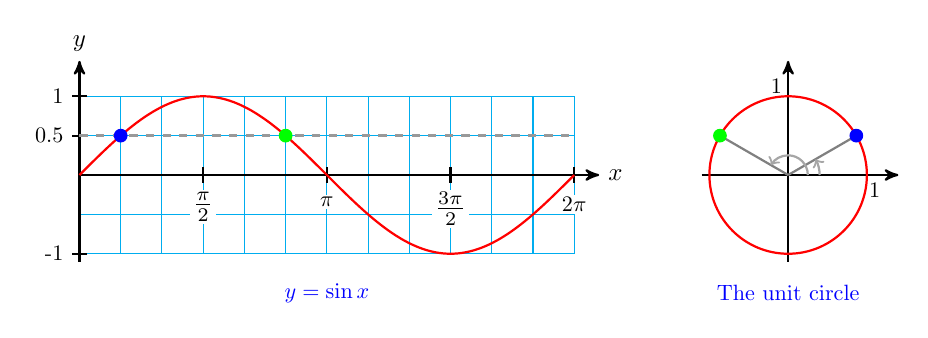
\begin{tikzpicture} 
\draw[cyan] (0,-1) grid[xstep=pi/6, ystep=1/2] (2*pi,1);
\draw[black,thick,->,>=stealth'] (0,0)--(6.6,0) node[right, scale=.9] {$x$};
\draw[black,thick,->,>=stealth'] (0,-1.1)--(0,1.45) node[above, scale=.9] {$y$};
\draw[black,thick] (pi/2,.1)--++(0,-.2) node[below, yshift=-2, fill=white, inner sep=1] {$\frac{\pi}{2}$};
\draw[black,thick] (pi,.1)--++(0,-.2) node[below, yshift=-4, fill=white, inner sep=1, scale=.8] {$\pi$};
\draw[black,thick] (3*pi/2,.1)--++(0,-.2) node[below, yshift=-2, fill=white, inner sep=1] {$\frac{3\pi}{2}$};
\draw[black,thick] (2*pi,.1)--++(0,-.2) node[below, yshift=-4, fill=white, inner sep=1, scale=.8] {$2\pi$};
\foreach \y in {-1, 0.5, 1} \draw[black,thick] (.1,\y)--++(-.2,0) node[left, scale=.8] {\y};
\draw[samples=65, domain=0:2*pi, variable=\x,smooth, red, thick] plot (\x,{ sin( deg(\x) });
\draw[gray!80!white, very thick, dashed] (0,0.5)--(2*pi,0.5);
\node[scale=.8, text=blue] at (pi,-1.5) {$y=\sin x$};
\filldraw[blue] (pi/6,1/2) circle (.08cm);
\filldraw[green] (5*pi/6,1/2) circle (.08cm);

%unit circle
\coordinate (O) at (9,0);
\coordinate (A) at ($ cos(30)*(1,0)+(9,1/2) $);
\coordinate (B) at ($ cos(150)*(1,0)+(9,1/2) $);
\draw[black,thick,->, >=stealth'] (O)++(-1.1,0)--++(2.5,0); 
\draw[black,thick,->, >=stealth'] (O)++(0,-1.1)--++(0,2.55); 
\draw[red,thick] (O) circle(1cm);
\draw[gray,thick] (O) --(A);
\draw[gray,thick] (O) --(B);
\draw[gray!70!white,thick,->] (9.4,0) arc(0:30:.4);
\draw[gray!70!white,thick,->] (9.25,0) arc(0:150:.25);
\node[scale=.8, text=blue] at (9,-1.5) {The unit circle};
\node[scale=.8] at (10.1,-.2) {1};
\node[scale=.8] at (8.85,1.13) {1};
\filldraw[blue] (A) circle (.08cm);
\filldraw[green] (B) circle (.08cm);

\end{tikzpicture}
\newline



fig-7-3-3 sine graph and unit circle

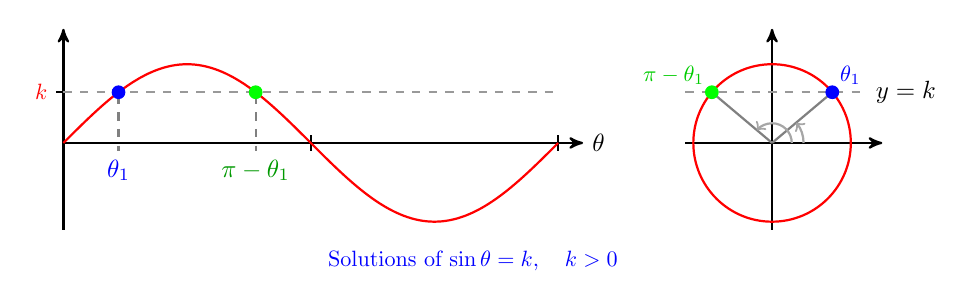
\begin{tikzpicture} 
\draw[black,thick,->,>=stealth'] (0,0)--(6.6,0) node[right, scale=.9] {$\theta$};
\draw[black,thick,->,>=stealth'] (0,-1.1)--(0,1.45);
\draw[gray,thick, dashed] (.7,{.6})--++(0,-.7) node[below, yshift=-2, fill=white, inner sep=1, scale=.9, text=blue] {$\theta_1$};
\draw[black,thick] (pi,.1)--++(0,-.2) ;
\draw[gray,thick, dashed] ({pi-.7},.6)--++(0,-.7) node[below, yshift=-2, fill=white, inner sep=1, scale=.9, text=green!60!black] {$\pi - \theta_1$};
\draw[black,thick] (2*pi,.1)--++(0,-.2);
\draw[black,thick] ($ (.1, 0) + sin(deg(.7)*(0,1) $)--++(-.2,0) node[left, scale=.8, text=red] {$k$};
\draw[samples=65, domain=0:2*pi, variable=\x,smooth, red, thick] plot (\x,{ sin( deg(\x) });
\draw[gray!80!white, thick, dashed] ($ sin(deg(.7)*(0,1) $)--++(2*pi,0);
\node[scale=.8, text=blue] at (5.2,-1.5) {Solutions of $\sin \theta=k, \quad k > 0$};
\filldraw[blue] ($ (.7, 0) + sin(deg(.7)*(0,1) $) circle (.08cm);
\filldraw[green] ($ ({pi-.7}, 0) + sin(deg(.7)*(0,1) $) circle (.08cm);

%unit circle
\coordinate (O) at (9,0);
\coordinate (A) at ($ cos(deg(.7))*(1,0)+(9,{sin(deg(.7))}) $);
\coordinate (B) at ($ cos(deg(.7))*(-1,0)+(9,{sin(deg(.7))}) $);
\draw[black,thick,->, >=stealth'] (O)++(-1.1,0)--++(2.5,0); 
\draw[black,thick,->, >=stealth'] (O)++(0,-1.1)--++(0,2.55); 
\draw[gray!80!white, thick, dashed] ($ sin(deg(.7)*(0,1) + (7.9,0) $)--++(2.3,0) node[right,text=black, scale=.9] {$y=k$};
\draw[red,thick] (O) circle(1cm);
\draw[gray,thick] (O) --(A);
\draw[gray,thick] (O) --(B);
\draw[gray!70!white,thick,->] (9.4,0) arc(0:{deg(.7)}:.4);
\draw[gray!70!white,thick,->] (9.25,0) arc(0:{deg(pi-.7)}:.25);
\filldraw[blue] (A) circle (.08cm);
\filldraw[green] (B) circle (.08cm);
\node[anchor=south west, scale=.8,text=blue] at (A) {$\theta_1$};
\node[anchor=south east, scale=.8, text=green!80!black] at (B) {$\pi - \theta_1$};
\end{tikzpicture}
\newline



fig-7-3-4 sine graph and unit circle

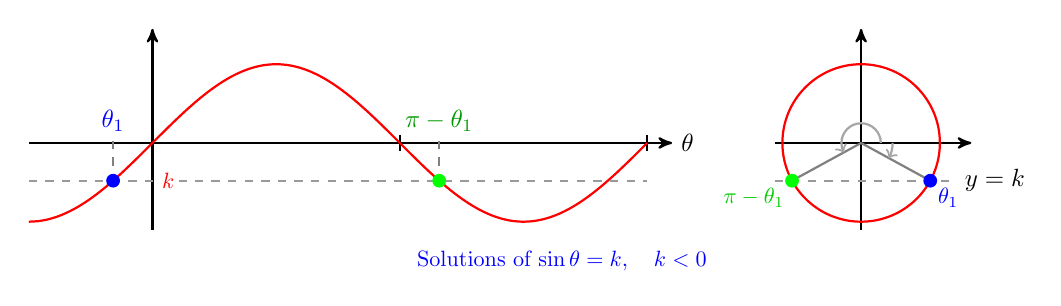
\begin{tikzpicture} 
\draw[black,thick,->,>=stealth'] (-pi/2,0)--(6.6,0) node[right, scale=.9] {$\theta$};
\draw[black,thick,->,>=stealth'] (0,-1.1)--(0,1.45);
\draw[gray,thick, dashed] (-.5,-{.5})--++(0,.6) node[above,  fill=white, inner sep=1, scale=.9, text=blue] {$\theta_1$};
\draw[black,thick] (pi,.1)--++(0,-.2) ;
\draw[gray,thick, dashed] ({pi+.5},-.5)--++(0,.6) node[above,  fill=white, inner sep=1, scale=.9, text=green!60!black] {$\pi - \theta_1$};
\draw[black,thick] (2*pi,.1)--++(0,-.2);
\draw[samples=65, domain=-pi/2:2*pi, variable=\x,smooth, red, thick] plot (\x,{ sin( deg(\x) });
\draw[gray!80!white, thick, dashed] ($ (-pi/2,0)+ sin(deg(.5)*(0,-1) $)--++(5*pi/2,0);
\node[scale=.8, text=blue] at (5.2,-1.5) {Solutions of $\sin \theta=k, \quad k < 0$};
\filldraw[blue] ($ (-.5, 0) + sin(deg(.5)*(0,-1) $) circle (.08cm);
\filldraw[green] ($ ({pi+.5}, 0) + sin(deg(.5)*(0,-1) $) circle (.08cm);
\node[fill=white, inner sep=2, text=red, scale=.8] at ($ (.2, 0) + sin(deg(.5)*(0,-1) $) {$k$};

%unit circle
\coordinate (O) at (9,0);
\coordinate (A) at ($ cos(deg(.5))*(1,0)+(9,{-sin(deg(.5))}) $);
\coordinate (B) at ($ cos(deg(.5))*(-1,0)+(9,{-sin(deg(.5))}) $);
\draw[black,thick,->, >=stealth'] (O)++(-1.1,0)--++(2.5,0); 
\draw[black,thick,->, >=stealth'] (O)++(0,-1.1)--++(0,2.55); 
\draw[gray!80!white, thick, dashed] ($ sin(deg(.5)*(0,-1) + (7.9,0) $)--++(2.3,0) node[right,text=black, scale=.9] {$y=k$};
\draw[red,thick] (O) circle(1cm);
\draw[gray,thick] (O) --(A);
\draw[gray,thick] (O) --(B);
\draw[gray!70!white,thick,->] (9.4,0) arc(0:{-deg(.5)}:.4);
\draw[gray!70!white,thick,->] (9.25,0) arc(0:{deg(pi+.5)}:.25);
\filldraw[blue] (A) circle (.08cm);
\filldraw[green] (B) circle (.08cm);
\node[anchor=north west, scale=.8,text=blue] at (A) {$\theta_1$};
\node[anchor=north east, scale=.8, text=green!80!black] at (B) {$\pi - \theta_1$};
\end{tikzpicture}
\newline



fig-7-3-5 cosine graph and unit circle

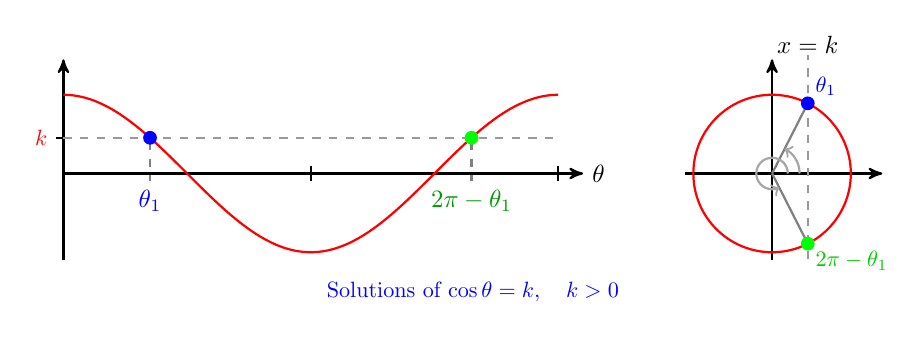
\begin{tikzpicture} 
\draw[black,thick,->,>=stealth'] (0,0)--(6.6,0) node[right, scale=.9] {$\theta$};
\draw[black,thick,->,>=stealth'] (0,-1.1)--(0,1.45);
\draw[gray,thick, dashed] (1.1,{.4})--++(0,-.5) node[below, yshift=-2, fill=white, inner sep=1, scale=.9, text=blue] {$\theta_1$};
\draw[black,thick] (pi,.1)--++(0,-.2) ;
\draw[gray,thick, dashed] ({2*pi-1.1},.4)--++(0,-.5) node[below, yshift=-2, fill=white, inner sep=1, scale=.9, text=green!60!black] {2$\pi - \theta_1$};
\draw[black,thick] (2*pi,.1)--++(0,-.2);
\draw[black,thick] ($ (.1, 0) + cos(deg(1.1)*(0,1) $)--++(-.2,0) node[left, scale=.8, text=red] {$k$};
\draw[samples=65, domain=0:2*pi, variable=\x,smooth, red, thick] plot (\x,{ cos( deg(\x) });
\draw[gray!80!white, thick, dashed] ($ cos(deg(1.1)*(0,1) $)--++(2*pi,0);
\node[scale=.8, text=blue] at (5.2,-1.5) {Solutions of $\cos \theta=k, \quad k > 0$};
\filldraw[blue] ($ (1.1, 0) + cos(deg(1.1)*(0,1) $) circle (.08cm);
\filldraw[green] ($ ({2*pi-1.1}, 0) + cos(deg(1.1)*(0,1) $) circle (.08cm);

%unit circle
\coordinate (O) at (9,0);
\coordinate (A) at ($ cos(deg(1.1))*(1,0)+(9,{sin(deg(1.1))}) $);
\coordinate (B) at ($ cos(deg(1.1))*(1,0)+(9,{-sin(deg(1.1))}) $);
\draw[black,thick,->, >=stealth'] (O)++(-1.1,0)--++(2.5,0); 
\draw[black,thick,->, >=stealth'] (O)++(0,-1.1)--++(0,2.55); 
\draw[gray!80!white, thick, dashed] ($ cos(deg(1.1)*(1,0) + (9,-0.2) +  sin(deg(-1.1)*(0,1)$)--++(0,2.6) node[above, yshift=-.1cm,text=black, scale=.9] {$x=k$};
\draw[red,thick] (O) circle(1cm);
\draw[gray,thick] (O) --(A);
\draw[gray,thick] (O) --(B);
\draw[gray!70!white,thick,->] (9.35,0) arc(0:{deg(1.1)}:.35);
\draw[gray!70!white,thick,->] (9.2,0) arc(0:{360-deg(1.1)}:.2);
\filldraw[blue] (A) circle (.08cm);
\filldraw[green] (B) circle (.08cm);
\node[anchor=south west, scale=.8,text=blue] at (A) {$\theta_1$};
\node[anchor=north west, scale=.8, text=green!80!black] at (B) {$2\pi - \theta_1$};
\end{tikzpicture}
\newline	



fig-7-3-6 cosine graph and unit circle

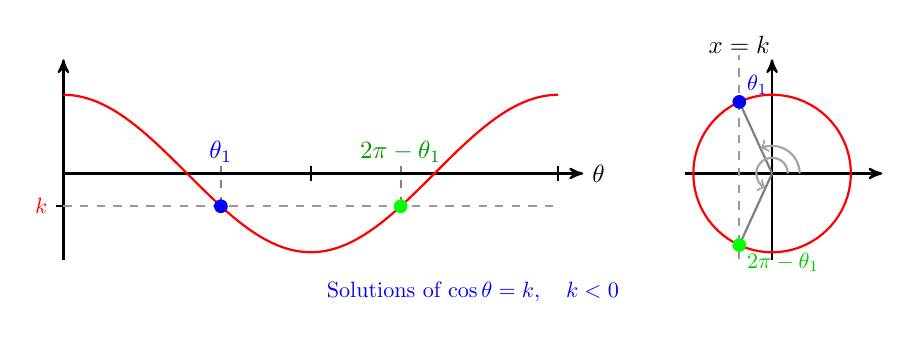
\begin{tikzpicture} 
\draw[black,thick,->,>=stealth'] (0,0)--(6.6,0) node[right, scale=.9] {$\theta$};
\draw[black,thick,->,>=stealth'] (0,-1.1)--(0,1.45);
\draw[gray,thick, dashed] (2,{-.4})--++(0,.5) node[above, yshift=0, fill=white, inner sep=1, scale=.9, text=blue] {$\theta_1$};
\draw[black,thick] (pi,.1)--++(0,-.2) ;
\draw[gray,thick, dashed] ({2*pi-2},-.4)--++(0,.5) node[above, yshift=0, fill=white, inner sep=1, scale=.9, text=green!60!black] {2$\pi - \theta_1$};
\draw[black,thick] (2*pi,.1)--++(0,-.2);
\draw[black,thick] ($ (.1, 0) + cos(deg(2)*(0,1) $)--++(-.2,0) node[left, scale=.8, text=red] {$k$};
\draw[samples=65, domain=0:2*pi, variable=\x,smooth, red, thick] plot (\x,{ cos( deg(\x) });
\draw[gray!80!white, thick, dashed] ($ cos(deg(2)*(0,1) $)--++(2*pi,0);
\node[scale=.8, text=blue] at (5.2,-1.5) {Solutions of $\cos \theta=k, \quad k < 0$};
\filldraw[blue] ($ (2, 0) + cos(deg(2)*(0,1) $) circle (.08cm);
\filldraw[green] ($ ({2*pi-2}, 0) + cos(deg(2)*(0,1) $) circle (.08cm);

%unit circle
\coordinate (O) at (9,0);
\coordinate (A) at ($ cos(deg(2))*(1,0)+(9,{sin(deg(2))}) $);
\coordinate (B) at ($ cos(deg(2))*(1,0)+(9,{-sin(deg(2))}) $);
\draw[black,thick,->, >=stealth'] (O)++(-1.1,0)--++(2.5,0); 
\draw[black,thick,->, >=stealth'] (O)++(0,-1.1)--++(0,2.55); 
\draw[gray!80!white, thick, dashed] ($ cos(deg(2)*(1,0) + (9,-0.2) +  sin(deg(-1.1)*(0,1)$)--++(0,2.6) node[above, yshift=-.1cm,text=black, scale=.9] {$x=k$};
\draw[red,thick] (O) circle(1cm);
\draw[gray,thick] (O) --(A);
\draw[gray,thick] (O) --(B);
\draw[gray!70!white,thick,->] (9.35,0) arc(0:{deg(2)}:.35);
\draw[gray!70!white,thick,->] (9.2,0) arc(0:{360-deg(2)}:.2);
\filldraw[blue] (A) circle (.08cm);
\filldraw[green] (B) circle (.08cm);
\node[anchor=south west, scale=.8,text=blue] at (A) {$\theta_1$};
\node[anchor=north west, scale=.8, text=green!80!black] at (B) {$2\pi - \theta_1$};
\end{tikzpicture}
\newline	


fig-7-3-7 tangent graph and slopes



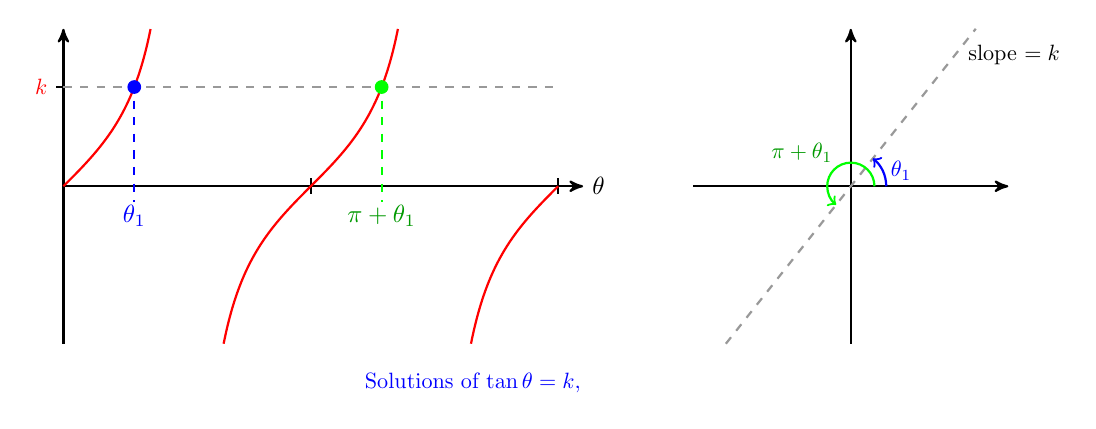
\begin{tikzpicture} 
\def\k{0.9};
\def\tank{tan(deg(\k))};
\draw[black,thick,->,>=stealth'] (0,0)--(6.6,0) node[right, scale=.9] {$\theta$};
\draw[black,thick,->,>=stealth'] (0,-2)--(0,2);
\draw[blue,thick, dashed] (\k,1.3)--++(0,-1.5) node[below, yshift=0, fill=white, inner sep=1, scale=.9, text=blue] {$\theta_1$};
\draw[black,thick] (pi,.1)--++(0,-.2) ;
\draw[green,thick, dashed] ({pi+\k},1.3)--++(0,-1.5) node[below, yshift=0, fill=white, inner sep=1, scale=.9, text=green!60!black] {$\pi + \theta_1$};
\draw[black,thick] (2*pi,.1)--++(0,-.2);
\draw[black,thick] ($ (.1, 0) + \tank*(0,1) $)--++(-.2,0) node[left, scale=.8, text=red] {$k$};
\draw[samples=65, domain=0:{atan(2)*pi/180}, variable=\x,smooth, red, thick] plot (\x,{ tan( deg(\x) });
\draw[samples=65, domain={-atan(2)*pi/180+pi}:{atan(2)*pi/180+pi}, variable=\x,smooth, red, thick] plot (\x,{ tan( deg(\x) });
\draw[samples=65, domain={-atan(2)*pi/180+2*pi}:{2*pi}, variable=\x,smooth, red, thick] plot (\x,{ tan( deg(\x) });
\draw[gray!80!white, thick, dashed] ($ \tank*(0,1) $)--++(2*pi,0);
\node[scale=.8, text=blue] at (5.2,-2.5) {Solutions of $\tan \theta=k, $};
\filldraw[blue] ($ (0.9, 0) + \tank *(0,1) $) circle (.08cm);
\filldraw[green] ($ ({pi+0.9}, 0) + \tank*(0,1) $) circle (.08cm);

%slope on second axis
\coordinate (O) at (10,0);
\coordinate (A) at ($ 2/ \tank *(1,0)+(10,2) $);
\coordinate (B) at ($ -2/ \tank *(1,0)+(10,-2) $);
\draw[black,thick,->, >=stealth'] (O)++(-2,0)--++(4,0); 
\draw[black,thick,->, >=stealth'] (O)++(0,-2)--++(0,4); 
\draw[gray!80!white, thick, dashed](B)--(A) node[below right, xshift=-.2cm, yshift=-.1cm,text=black, scale=.8] {slope $=k$};
%\draw[green,thick, dashed] (O) --(B);
\draw[blue,thick,->] (10.45,0) arc(0:{deg(\k)}:.45) node[right, midway, scale=.8]  {$\theta_1$};
\draw[green,thick,->] (10.3,0) arc(0:{180+deg(\k)}:.3) node[above left, yshift=-2, midway, scale=.8, text=green!60!black]  {$\pi+\theta_1$};;
\end{tikzpicture}
\newline	




fig-7-3-8 sin 2x graph and unit circle

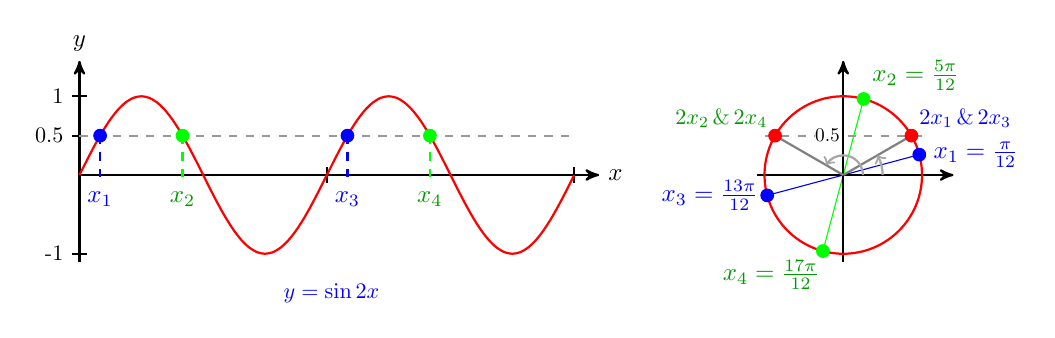
\begin{tikzpicture} 
\draw[black,thick,->,>=stealth'] (0,0)--(6.6,0) node[right, scale=.9] {$x$};
\draw[black,thick,->,>=stealth'] (0,-1.1)--(0,1.45) node[above, scale=.9] {$y$};
\foreach \y in {-1, 0.5, 1} \draw[black,thick] (.1,\y)--++(-.2,0) node[left, scale=.8] {\y};
\draw[blue,thick, dashed] (pi/12,0.5)--++(0,-.6) node[below,scale=.9]{$x_1$};
\draw[green,thick, dashed, text=green!60!black] ({5*pi/12},0.5)--++(0,-.6)  node[below,scale=.9]{$x_2$};
\draw[blue,thick, dashed] (13*pi/12,0.5)--++(0,-.6) node[below,scale=.9]{$x_3$};
\draw[green,thick, dashed, text=green!60!black] ({17*pi/12},0.5)--++(0,-.6)  node[below,scale=.9]{$x_4$};
\draw[black,thick] (pi,.1)--++(0,-.2) ;
\draw[black,thick] (2*pi,.1)--++(0,-.2);
\draw[samples=65, domain=0:2*pi, variable=\x,smooth, red, thick] plot (\x,{ sin( deg(2*\x) });
\draw[gray!80!white, thick, dashed] (0,0.5)--++(2*pi,0);
\node[scale=.8, text=blue] at (3.2,-1.5) {$y=\sin 2x$};
\filldraw[blue] (pi/12, 0.5) circle (.08cm);
\filldraw[green] (5*pi/12,0.5) circle (.08cm);
\filldraw[blue] (13*pi/12, 0.5) circle (.08cm);
\filldraw[green] (17*pi/12,0.5) circle (.08cm);

%unit circle
\def\del{9.7};
\coordinate (O) at (\del,0);
\coordinate (A) at ($ sqrt(3)*(1/2,0)+(\del,0.5) $);
\coordinate (B) at ($ -sqrt(3)*(1/2,0)+(\del,0.5) $);
\coordinate (x1) at ($ cos(15)*(1,0)+(\del,0) + sin(15)*(0,1)$);
\coordinate (x3) at ($ cos(15)*(-1,0)+(\del,0) + sin(15)*(0,-1)$);
\draw[blue] (x1)--(x3);
\coordinate (x2) at ($ cos(75)*(1,0)+(\del,0) + sin(75)*(0,1)$);
\coordinate (x4) at ($ cos(75)*(-1,0)+(\del,0) + sin(75)*(0,-1)$);
\draw[green] (x2)--(x4);
\draw[black,thick,->, >=stealth'] (O)++(-1.1,0)--++(2.5,0); 
\draw[black,thick,->, >=stealth'] (O)++(0,-1.1)--++(0,2.55); 
\draw[gray!80!white, thick, dashed] ($ \del*(1,0)+(0,0.5) + (-1.,0) $)--++(2.,0) ;
\draw[red,thick] (O) circle(1cm);
\draw[gray,thick] (O) --(A);
\draw[gray,thick] (O) --(B);
\draw[gray!70!white,thick,->] ($ \del*(1,0) +(.5,0)$) arc(0:30:.5);
\draw[gray!70!white,thick,->] ($ \del*(1,0) +(.25,0)$) arc(0:150:.25);
\filldraw[blue] (x1) circle (.08cm) node[right, xshift=2, scale=.9] {$x_1=\frac{\pi}{12}$};
\filldraw[blue] (x3) circle (.08cm) node[left, scale=.9] {$x_3=\frac{13\pi}{12}$};
\filldraw[green] (x2) circle (.08cm) node[above right, text=green!60!black, scale=.9] {$x_2=\frac{5\pi}{12}$};
\filldraw[green] (x4) circle (.08cm) node[below left, xshift=2, text=green!60!black, scale=.9] {$x_4=\frac{17\pi}{12}$};
\filldraw[red] (A) circle (.08cm);
\filldraw[red] (B) circle (.08cm);
\node[anchor=south west, scale=.8,text=blue] at (A) {$2x_1\, \& \, 2x_3$};
\node[anchor=south east, scale=.8, text=green!60!black] at (B) {$2x_2\, \& \, 2x_4$};
\node[fill=white, inner sep=0, scale=.7] at ($ (\del,0) + (-.2,0.5) $) {$0.5$};
\end{tikzpicture}
\newline



exer7-3-2ans a.k.a. ar7-3-2ans

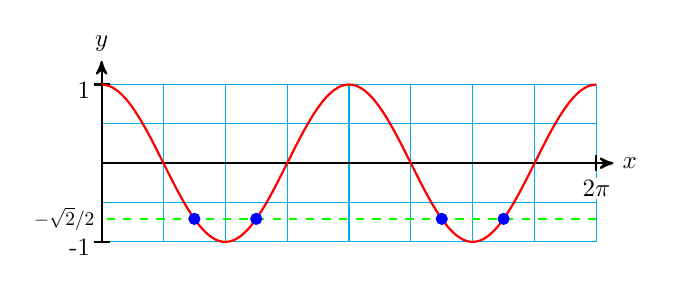
\begin{tikzpicture}
\draw[cyan] (0,-1) grid[xstep=pi/4, ystep=1/2] (2*pi,1);
\draw[black,thick,->,>=stealth'] (0,0) -- (6.5,0) node[right,scale=.9] {$x$};
\draw[black,thick] (2*pi,.1)--++(0,-.2) node[below, yshift=-2, fill=white, inner sep=1, scale=.9] {$2\pi$};
\draw[black,thick,->,>=stealth'] (0,-1) -- (0,1.3) node[above,scale=.9] {$y$};
\foreach \y in {-1,1} \draw[black,thick] (.1,\y)--++(-.2,0) node[left, xshift=2, yshift=-2, scale=.9]{\y};
\draw[samples=65,domain=0:2*pi, variable=\x, smooth, red, thick] plot(\x,{cos(deg(2*\x))});
\coordinate (C) at ($ 1/sqrt(2)*(0, -1) $);
\coordinate (D) at ($ 1/sqrt(2)*(0, -1)+(2*pi,0) $);
\draw[green, thick, dashed] (D)--(C) node[left, scale=.7, text=black] {$-\sqrt{2}/2$};
\filldraw[blue] ($ 1/sqrt(2)*(0,-1)+(3*pi/8,0) $) circle (.07cm);
\filldraw[blue] ($ 1/sqrt(2)*(0,-1)+(5*pi/8,0) $) circle (.07cm);
\filldraw[blue] ($ 1/sqrt(2)*(0,-1)+(11*pi/8,0) $) circle (.07cm);
\filldraw[blue] ($ 1/sqrt(2)*(0,-1)+(13*pi/8,0) $) circle (.07cm);
\end{tikzpicture}
\newline



exam7-3-3 tan 2t

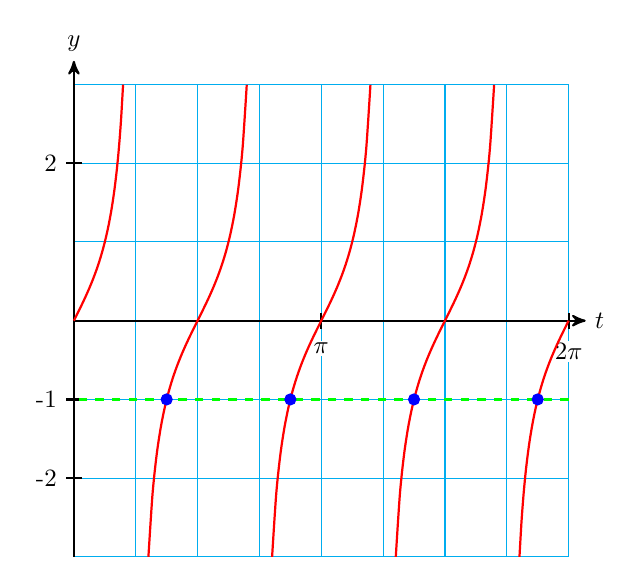
\begin{tikzpicture}
\draw[cyan] (0,-3) grid[xstep=pi/4] (2*pi,3);
\draw[black,thick,->,>=stealth'] (0,0) -- (6.5,0) node[right,scale=.9] {$t$};
\draw[black,thick] (pi,.1)--++(0,-.2) node[below, yshift=-4, fill=white, inner sep=1, scale=.9] {$\pi$};
\draw[black,thick] (2*pi,.1)--++(0,-.2) node[below, yshift=-4, fill=white, inner sep=1, scale=.9] {$2\pi$};
\draw[black,thick,->,>=stealth'] (0,-3) -- (0,3.3) node[above,scale=.9] {$y$};
\foreach \y in {-2,2,-1} \draw[black,thick] (.1,\y)--++(-.2,0) node[left, scale=.9]{\y};
\draw[domain=0:{atan(3)*pi/360}, variable=\x, smooth, red, thick] plot(\x,{tan(deg(2*\x))});
\draw[domain={pi/2-atan(3)*pi/360}:{pi/2+atan(3)*pi/360}, variable=\x, smooth, red, thick] plot(\x,{tan(deg(2*\x))});
\draw[domain={pi-atan(3)*pi/360}:{pi+atan(3)*pi/360}, variable=\x, smooth, red, thick] plot(\x,{tan(deg(2*\x))});
\draw[domain={3*pi/2-atan(3)*pi/360}:{3*pi/2+atan(3)*pi/360}, variable=\x, smooth, red, thick] plot(\x,{tan(deg(2*\x))});
\draw[domain={2*pi-atan(3)*pi/360}:2*pi, variable=\x, smooth, red, thick] plot(\x,{tan(deg(2*\x))});
\draw[green, thick, dashed] (2*pi,-1)--++(-2*pi,0);
\filldraw[blue] (3*pi/8,-1) circle (.07cm);
\filldraw[blue] (7*pi/8,-1) circle (.07cm);
\filldraw[blue] (11*pi/8,-1) circle (.07cm);
\filldraw[blue] (15*pi/8,-1) circle (.07cm);
\end{tikzpicture}
\newline



fig-7-3-9

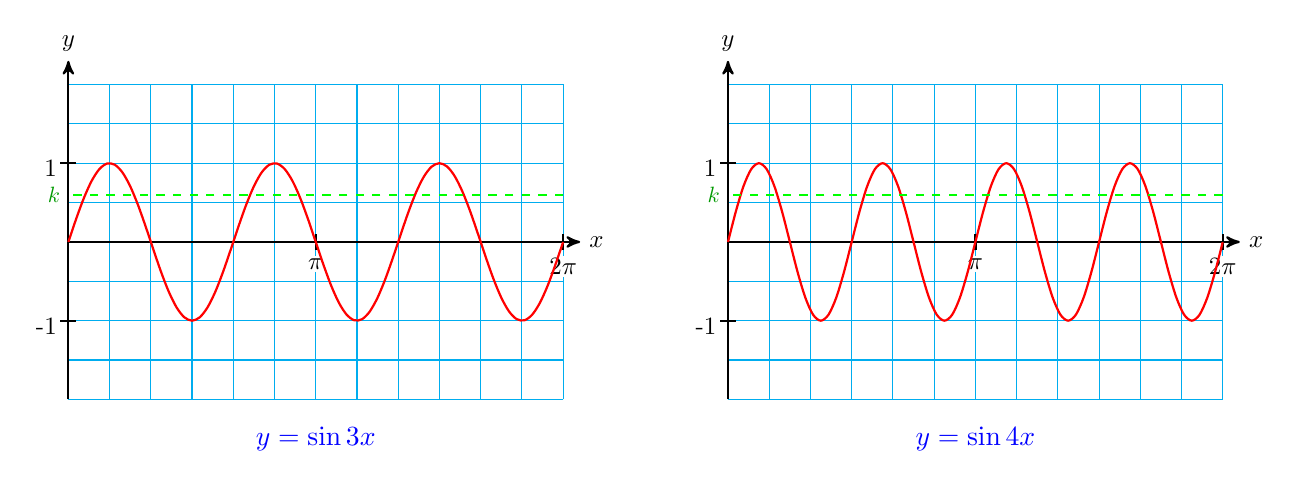
\begin{tikzpicture}
\draw[cyan] (0,-2) grid[xstep=pi/6, ystep=1/2] (2*pi,2);
\draw[black,thick,->,>=stealth'] (0,0) -- (6.5,0) node[right,scale=.9] {$x$};
\draw[black,thick,->,>=stealth'] (0,-2) -- (0,2.3) node[above,scale=.9] {$y$};
\draw[black,thick] (pi,.1)--++(0,-.2) node[below, yshift=-2, fill=white, inner sep=1, scale=.9] {$\pi$};
\draw[black,thick] (2*pi,.1)--++(0,-.2) node[below, yshift=-2, fill=white, inner sep=1, scale=.9] {$2\pi$};
\foreach \y in {-1,1} \draw[black,thick] (.1,\y)--++(-.2,0) node[left, xshift=2, yshift=-2, scale=.9]{\y};
\draw[samples=65,domain=0:2*pi, variable=\x, smooth, red, thick] plot(\x,{sin(deg(3*\x))});
\def\k{.6};
\node[text=blue] at (pi,-2.5) {$y=\sin 3x$};
\coordinate (C) at (0,\k) ;
\coordinate (D) at (2*pi,\k) ;
\draw[green,thick,dashed] (D)--(C) node[left,scale=.8, text=green!60!black] {$k$};

%second grid
\def\del{8*pi/3};
\coordinate (O) at ($ \del*(1,0) $);
\draw[cyan] ($ \del*(1,0) +(0,-2) $) grid[xstep=pi/6, ystep=1/2] ($ \del*(1,0) +(2*pi,2) $);
\draw[black,thick,->,>=stealth'] (O) --++ (6.5,0) node[right,scale=.9] {$x$};
\draw[black,thick,->,>=stealth'] ($ \del*(1,0) +(0,-2)$) --++ (0,4.3) node[above,scale=.9] {$y$};
\draw[black,thick] ($ \del*(1,0) +(pi,.1)$)--++(0,-.2) node[below, yshift=-2, fill=white, inner sep=1, scale=.9] {$\pi$};
\draw[black,thick] ($ \del*(1,0) +(2*pi,.1)$)--++(0,-.2) node[below, yshift=-2, fill=white, inner sep=1, scale=.9] {$2\pi$};
\foreach \y in {-1,1} \draw[black,thick] ($ \del*(1,0) +(.1,\y)$)--++(-.2,0) node[left, xshift=2, yshift=-2, scale=.9]{\y};
\draw[samples=65,domain=0:2*pi, variable=\x, smooth, red, thick] plot({\x+\del},{sin(deg(4*\x))});
\def\k{.6};
\node[text=blue] at ($ \del*(1,0) +(pi,-2.5)$) {$y=\sin 4x$};
\coordinate (C) at ($ \del*(1,0)+(0,\k) $);
\coordinate (D) at ($ \del*(1,0)+(2*pi,\k)$) ;
\draw[green,thick,dashed] (D)--(C) node[left,scale=.8, text=green!60!black] {$k$};
\end{tikzpicture}
\newline



exam7-3-6  5 + 0.4 tan (3x-0.5)

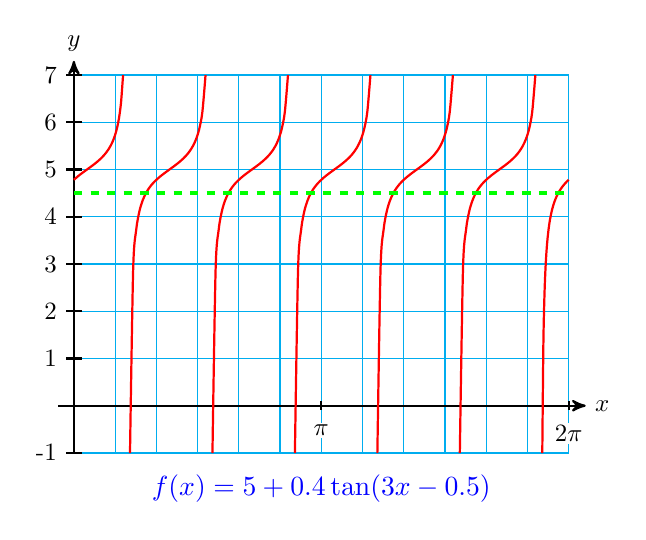
\begin{tikzpicture} [yscale=.6]
\draw[cyan] (0,-1) grid[xstep=pi/6] (2*pi,7);
\draw[black,thick,->,>=stealth'] (-0.2,0) -- (6.5,0) node[right,scale=.9] {$x$};
\draw[black,thick,->,>=stealth'] (0,-1) -- (0,7.3) node[above,scale=.9] {$y$};
\draw[black,thick] (pi,.1)--++(0,-.2) node[below, yshift=-4, fill=white, inner sep=1, scale=.9] {$\pi$};
\draw[black,thick] (2*pi,.1)--++(0,-.2) node[below, yshift=-4, fill=white, inner sep=1, scale=.9] {$2\pi$};
\foreach \y in {-1,5,1,2,3,4,6,7} \draw[black,thick] (.1,\y)--++(-.2,0) node[left, scale=.9]{\y};
\draw[domain=0:{atan(5)*pi/540+0.5/3}, variable=\x, smooth, red, thick] plot({\x},{5+0.4*tan(deg(3*\x-0.5 ))});
\draw[domain={atan(-15)*pi/540+0.5/3 +pi/3}:{atan(5)*pi/540+0.5/3+pi/3}, variable=\x, smooth, red, thick] plot({\x+pi/3},{5+0.4*tan(deg(3*\x-0.5 ))});
\draw[domain={atan(-15)*pi/540+0.5/3 +pi/3}:{atan(5)*pi/540+0.5/3+pi/3}, variable=\x, smooth, red, thick] plot({\x},{5+0.4*tan(deg(3*\x-0.5 ))});
\draw[domain={atan(-15)*pi/540+0.5/3 +pi/3}:{atan(5)*pi/540+0.5/3+pi/3}, variable=\x, smooth, red, thick] plot({\x+2*pi/3},{5+0.4*tan(deg(3*\x-0.5 ))});
\draw[domain={atan(-15)*pi/540+0.5/3 +pi/3}:{atan(5)*pi/540+0.5/3+pi/3}, variable=\x, smooth, red, thick] plot({\x+pi},{5+0.4*tan(deg(3*\x-0.5 ))});
\draw[domain={atan(-15)*pi/540+0.5/3 +pi/3}:{atan(5)*pi/540+0.5/3+pi/3}, variable=\x, smooth, red, thick] plot({\x+4*pi/3},{5+0.4*tan(deg(3*\x-0.5 ))});
\draw[domain={atan(-15)*pi/540+0.5/3 +pi/3}:{pi/3}, variable=\x, smooth, red, thick] plot({\x+5*pi/3},{5+0.4*tan(deg(3*\x-0.5 ))});
\draw[green, very thick, dashed] (0,4.5)--++(2*pi,0);
\node[text=blue] at (pi,-1.75) {$f(x) = 5+0.4 \tan(3x-0.5)$};
\end{tikzpicture}
\newline



exer7-3-6ans a.k.a. ar7-3-6ans 2-4 tan 3(x+0.2)

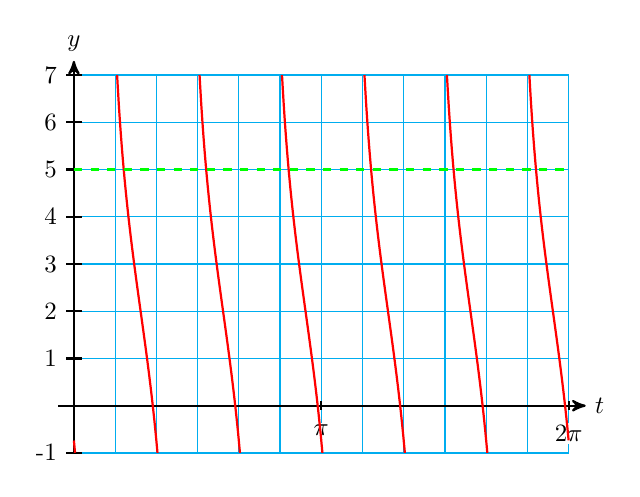
\begin{tikzpicture} [yscale=.6]
\draw[cyan] (0,-1) grid[xstep=pi/6] (2*pi,7);
\draw[black,thick,->,>=stealth'] (-0.2,0) -- (6.5,0) node[right,scale=.9] {$t$};
\draw[black,thick,->,>=stealth'] (0,-1) -- (0,7.3) node[above,scale=.9] {$y$};
\draw[black,thick] (pi,.1)--++(0,-.2) node[below, yshift=-4, fill=white, inner sep=1, scale=.9] {$\pi$};
\draw[black,thick] (2*pi,.1)--++(0,-.2) node[below, yshift=-4, fill=white, inner sep=1, scale=.9] {$2\pi$};
\foreach \y in {-1,5,1,2,3,4,6,7} \draw[black,thick] (.1,\y)--++(-.2,0) node[left, scale=.9]{\y};
\draw[domain={atan(-5/4)*pi/540-0.2+pi/3}:{atan(3/4)*pi/540-0.2+pi/3}, variable=\x, smooth, red, thick] plot({\x},{2-4*tan(deg(3*(\x+0.2) ))});
\draw[domain={atan(-5/4)*pi/540-0.2+pi/3}:{atan(3/4)*pi/540-0.2+pi/3}, variable=\x, smooth, red, thick] plot({\x+pi/3},{2-4*tan(deg(3*(\x+0.2) ))});
\draw[domain={atan(-5/4)*pi/540-0.2+pi/3}:{atan(3/4)*pi/540-0.2+pi/3}, variable=\x, smooth, red, thick] plot({\x+2*pi/3},{2-4*tan(deg(3*(\x+0.2) ))});
\draw[domain={atan(-5/4)*pi/540-0.2+pi/3}:{atan(3/4)*pi/540-0.2+pi/3}, variable=\x, smooth, red, thick] plot({\x+pi},{2-4*tan(deg(3*(\x+0.2) ))});
\draw[domain={atan(-5/4)*pi/540-0.2+pi/3}:{atan(3/4)*pi/540-0.2+pi/3}, variable=\x, smooth, red, thick] plot({\x+4*pi/3},{2-4*tan(deg(3*(\x+0.2) ))});
\draw[domain=0:{atan(3/4)*pi/540-0.2}, variable=\x, smooth, red, thick] plot({\x},{2-4*tan(deg(3*(\x+0.2) ))});
\draw[domain={atan(-5/4)*pi/540-0.2+pi/3}:{pi/3}, variable=\x, smooth, red, thick] plot({\x+5*pi/3},{2-4*tan(deg(3*(\x+0.2) ))});
\draw[green, very thick, dashed] (0,5)--++(2*pi,0);
\end{tikzpicture}
\newline



exam7-3-7 -8sin(2000 pi t) +8

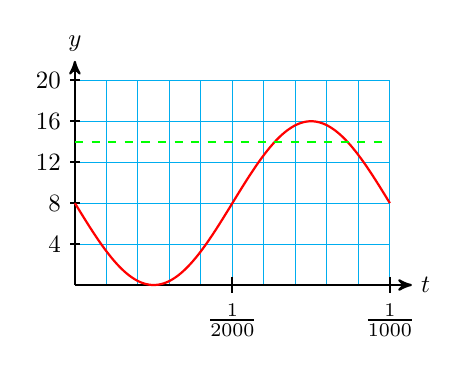
\begin{tikzpicture} [xscale=.4,yscale=.13]
\draw[cyan] (0,0) grid[ystep=4] (10,20);
\draw[black,thick,->,>=stealth'] (0,0)--(10.7,0) node[right, scale=.9] {$t$};
\draw[black,thick,->,>=stealth'] (0,0)--(0,21.9) node[above, scale=.9] {$y$};
\foreach \y in {4,8,12,16,20} \draw[black,thick] (.15,\y)--++(-.3,0) node[left,scale=.9] {\y};
\draw[black,thick] (5,.8)--++(0,-1.6) node[below] {$\frac{1}{2000}$};
\draw[black,thick] (10,.8)--++(0,-1.6) node[below] {$\frac{1}{1000}$};
\draw[samples=65,domain=0:10, variable=\t, smooth, red, thick] plot(\t, {8-8*sin( 36*\t )});
\draw[green,thick,dashed] (0,14)--++(10,0);
\end{tikzpicture}
\newline



hp7-3-43ans $P(t)=4000\cos(\frac{\pi}{6}t)+46,000$

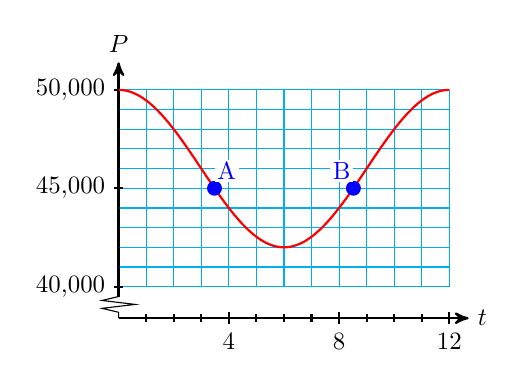
\begin{tikzpicture} [xscale=.35,yscale=.25]
\draw[cyan] (0,40) grid[ystep=1] (12,50);
\draw[black,thick,->,>=stealth'] (0,38.4)--++(12.7,0) node[right, scale=.9] {$t$};
\draw[black,thick,->,>=stealth'] (0,39.5)--++(0,11.9) node[above, scale=.9] {$P$};
\foreach \x in {1,2,...,12} \draw[black,thick] (\x,38.6)--++(0,-.4);
\foreach \x in {4,8,12} \draw[black,thick] (\x,38.7)--++(0,-.6) node[below, scale=.9] {\x};
\coordinate (O) at (0,39.5);
\draw[black] (O)--++(-.6, -.2)--++(1.2,-.2)--++(-1.2,-.2)--++(.6,-.2) -- ++(0, -.3);
\draw[black,thick] (.15,40)--++(-.3,0) node[left,scale=.9] {40,000};
\draw[black,thick] (.15,45)--++(-.3,0) node[left,scale=.9] {45,000};
\draw[black,thick] (.15,50)--++(-.3,0) node[left,scale=.9] {50,000};
\draw[samples=65,domain=0:12, variable=\t, smooth, red, thick] plot(\t, {( 46+4*cos(30*\t )});
\filldraw[blue] (3.48,45) ellipse(.25cm and .35cm) node[above right, yshift=2,scale=.9, fill=white, inner sep=1] {A};
\filldraw[blue] (8.52,45) ellipse(.25cm and .35cm) node[above left, yshift=2,scale=.9, fill=white, inner sep=1] {B};
\end{tikzpicture}
\newline



hp7-3-45ans $h(t)=11-10\cos(\frac{\pi}{30}t)$

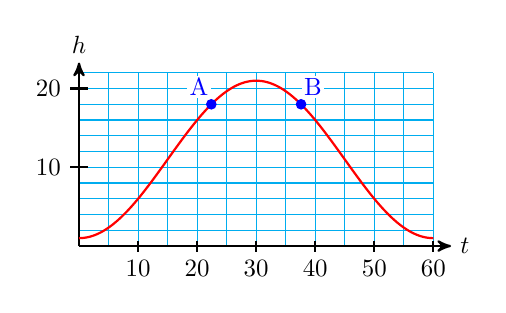
\begin{tikzpicture} [xscale=.075,yscale=.1]
\draw[cyan] (0,0) grid[xstep=5,ystep=2] (60,22);
\draw[black,thick,->,>=stealth'] (0,0)--++(63,0) node[right, scale=.9] {$t$};
\draw[black,thick,->,>=stealth'] (0,0)--++(0,23.3) node[above, scale=.9] {$h$};
\foreach \x in {10,20,...,60} \draw[black,thick] (\x,.7)--++(0,-1.4) node[below, scale=.9] {\x};
\foreach \y in {10,20} \draw[black,thick] (1.5,\y)--++(-3,0) node[left,scale=.9] {\y};
\draw[samples=65,domain=0:60, variable=\t, smooth, red, thick] plot(\t, { 11-10*cos(6*\t )});
\filldraw[blue] (22.4,18) ellipse(.8cm and .6cm) node[above left, yshift=2,scale=.9, fill=white, inner sep=1] {A};
\filldraw[blue] (37.6,18) ellipse(.8cm and .6cm) node[above right, yshift=2,scale=.9, fill=white, inner sep=1] {B};
\end{tikzpicture}
\newline


hp7-sum-5ans  $y=2+3\cos t$

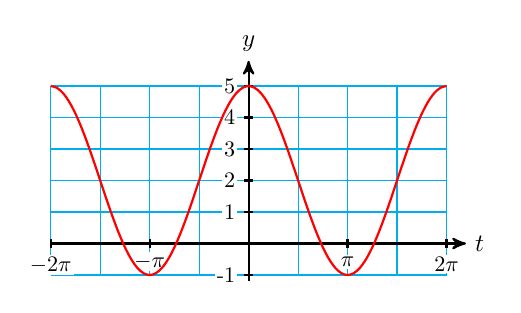
\begin{tikzpicture} [scale=.4]
\draw[cyan] (-2*pi,-1) grid[xstep=pi/2] (2*pi,5);
\draw[black,thick,->,>=stealth'] (-2*pi,0)--(6.9,0) node[right, scale=.9] {$t$};
\draw[black,thick,->,>=stealth'] (0,-1.2)--(0,5.8) node[above, scale=.9] {$y$};
\draw[black,thick] (-2*pi,.15)--++(0,-.3) node[below, yshift=-2, fill=white, inner sep=1, scale=.8] {$-2\pi$};
\draw[black,thick] (-pi,.15)--++(0,-.3) node[below, yshift=-1, fill=white, inner sep=1, scale=.8] {$-\pi$};
\draw[black,thick] (2*pi,.15)--++(0,-.3) node[below, yshift=-2, fill=white, inner sep=1, scale=.8] {$2\pi$};
\draw[black,thick] (pi,.15)--++(0,-.3) node[below, yshift=-2, fill=white, inner sep=1, scale=.8] {$\pi$};
\foreach \y in {-1,1,2,...,5} \draw[black,thick] (.15,\y)--++(-.3,0) node[left, xshift=-2, fill=white, inner sep=1, scale=.8] {\y};
\draw[samples=65,domain=-2*pi:2*pi, variable=\t, smooth, red, thick] plot (\t,{2+3*cos(deg(\t))});
\end{tikzpicture}
\newline


hp7-sum-7ans  $y=-4\sin \pi w$

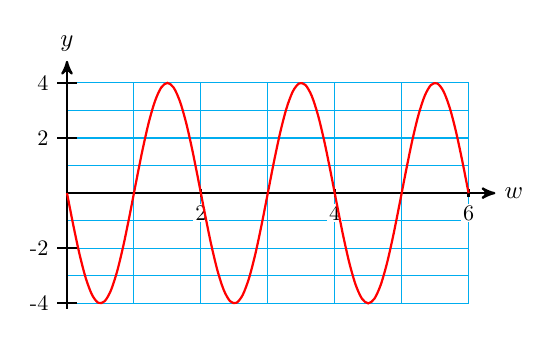
\begin{tikzpicture} [xscale=.85, yscale=.35]
\draw[cyan] (0,-4) grid[xstep=1] (6,4);
\draw[black,thick,->,>=stealth'] (0,0)--(6.4,0) node[right, scale=.9] {$w$};
\draw[black,thick,->,>=stealth'] (0,-4.2)--(0,4.8) node[above, scale=.9] {$y$};
\foreach \x in {2,4,6} \draw[black,thick] (\x,.15)--++(0,-.3) node[below, yshift=-2, fill=white, inner sep=1, scale=.8] {\x};
\foreach \y in {-4,-2,2,4} \draw[black,thick] (.15,\y)--++(-.3,0) node[left, xshift=-2, fill=white, inner sep=1, scale=.8] {\y};
\draw[samples=65,domain=-0:6, variable=\t, smooth, red, thick] plot (\t,{-4*sin(deg(pi*\t))});
\end{tikzpicture}
\newline



hp7-sum-9 $y=3+2\sin x$

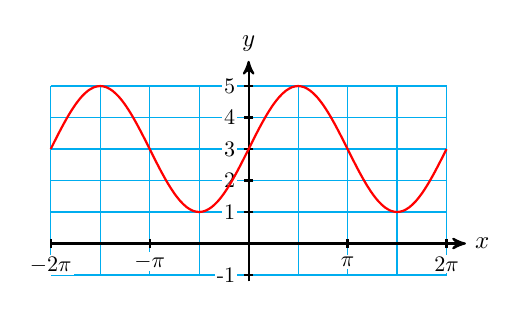
\begin{tikzpicture} [scale=.4]
\draw[cyan] (-2*pi,-1) grid[xstep=pi/2] (2*pi,5);
\draw[black,thick,->,>=stealth'] (-2*pi,0)--(6.9,0) node[right, scale=.9] {$x$};
\draw[black,thick,->,>=stealth'] (0,-1.2)--(0,5.8) node[above, scale=.9] {$y$};
\draw[black,thick] (-2*pi,.15)--++(0,-.3) node[below, yshift=-2, fill=white, inner sep=1, scale=.8] {$-2\pi$};
\draw[black,thick] (-pi,.15)--++(0,-.3) node[below, yshift=-1, fill=white, inner sep=1, scale=.8] {$-\pi$};
\draw[black,thick] (2*pi,.15)--++(0,-.3) node[below, yshift=-2, fill=white, inner sep=1, scale=.8] {$2\pi$};
\draw[black,thick] (pi,.15)--++(0,-.3) node[below, yshift=-2, fill=white, inner sep=1, scale=.8] {$\pi$};
\foreach \y in {-1,1,2,...,5} \draw[black,thick] (.15,\y)--++(-.3,0) node[left, xshift=-2, fill=white, inner sep=1, scale=.8] {\y};
\draw[samples=65,domain=-2*pi:2*pi, variable=\t, smooth, red, thick] plot (\t,{3+2*sin(deg(\t))});
\end{tikzpicture}
\newline



hp7-sum-10 $y=-2+3\cos x$

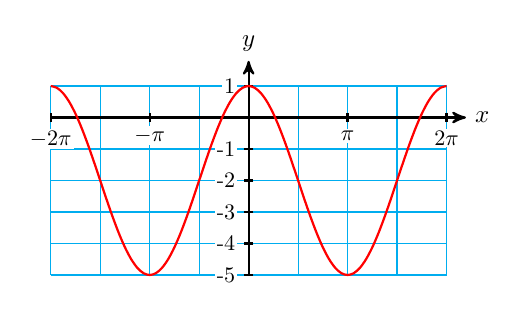
\begin{tikzpicture} [scale=.4]
\draw[cyan] (-2*pi,-5) grid[xstep=pi/2] (2*pi,1);
\draw[black,thick,->,>=stealth'] (-2*pi,0)--(6.9,0) node[right, scale=.9] {$x$};
\draw[black,thick,->,>=stealth'] (0,-5)--(0,1.8) node[above, scale=.9] {$y$};
\draw[black,thick] (-2*pi,.15)--++(0,-.3) node[below, yshift=-2, fill=white, inner sep=1, scale=.8] {$-2\pi$};
\draw[black,thick] (-pi,.15)--++(0,-.3) node[below, yshift=-1, fill=white, inner sep=1, scale=.8] {$-\pi$};
\draw[black,thick] (2*pi,.15)--++(0,-.3) node[below, yshift=-2, fill=white, inner sep=1, scale=.8] {$2\pi$};
\draw[black,thick] (pi,.15)--++(0,-.3) node[below, yshift=-2, fill=white, inner sep=1, scale=.8] {$\pi$};
\foreach \y in {-5,-4,...,-1,1} \draw[black,thick] (.15,\y)--++(-.3,0) node[left, xshift=-2, fill=white, inner sep=1, scale=.8] {\y};
\draw[samples=65,domain=-2*pi:2*pi, variable=\t, smooth, red, thick] plot (\t,{-2+3*cos(deg(\t))});
\end{tikzpicture}
\newline



hp7-sum-11 $y=4-3\sin \frac{x}{4}$

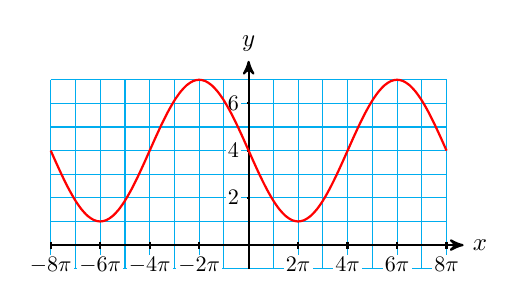
\begin{tikzpicture} [xscale=.1,yscale=.3]
\draw[cyan] (-8*pi,-1) grid[xstep=pi] (8*pi,7);
\draw[black,thick,->,>=stealth'] (-8*pi,0)--(27.3,0) node[right, scale=.9] {$x$};
\draw[black,thick,->,>=stealth'] (0,-1)--(0,7.8) node[above, scale=.9] {$y$};
\foreach \x [evaluate=\x as \xi using (pi*\x)]  in {-8,-6,-4,-2,2,4,6,8}  \draw[black,thick] (\xi,.15)--++(0,-.3) node[below, yshift=-2, fill=white, inner sep=1, scale=.8] {$\x \pi$};
\foreach \y in {2,4,6} \draw[black,thick] (.15,\y)--++(-.3,0) node[left, xshift=-2, fill=white, inner sep=1, scale=.8] {\y};
\draw[samples=65,domain=-8*pi:8*pi, variable=\t, smooth, red, thick] plot (\t,{4-3*sin(deg(\t)/4)});
\end{tikzpicture}
\newline



hp7-sum-12 $y=2-4\cos 8x$

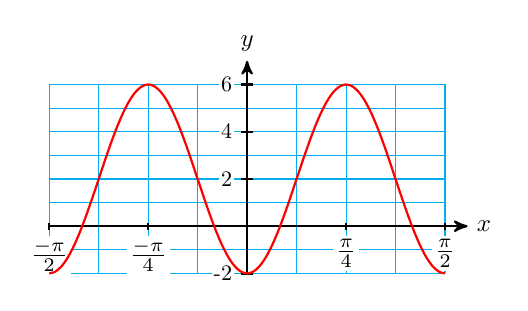
\begin{tikzpicture} [xscale=1.6,yscale=.3]
\draw[cyan] (-pi/2,-2) grid[xstep=pi/8] (pi/2,6);
\draw[black,thick,->,>=stealth'] (-pi/2,0)--(1.75,0) node[right, scale=.9] {$x$};
\draw[black,thick,->,>=stealth'] (0,-2)--(0,7.) node[above, scale=.9] {$y$};
\draw[black,thick] (-pi/2,.15)--++(0,-.3) node[below, yshift=-2, fill=white, inner sep=1] {$\frac{-\pi}{2}$};
\draw[black,thick] (-pi/4,.15)--++(0,-.3) node[below, yshift=-2, fill=white, inner sep=1] {$\frac{-\pi}{4}$};
\draw[black,thick] (pi/4,.15)--++(0,-.3) node[below, yshift=-2, fill=white, inner sep=1] {$\frac{\pi}{4}$};
\draw[black,thick] (pi/2,.15)--++(0,-.3) node[below, yshift=-2, fill=white, inner sep=1] {$\frac{\pi}{2}$};
\foreach \y in {-2,2,4,6} \draw[black,thick] (.05,\y)--++(-.1,0) node[left, xshift=-2, fill=white, inner sep=1, scale=.8] {\y};
\draw[samples=65,domain=-pi/2:pi/2, variable=\t, smooth, red, thick] plot (\t,{2-4*cos(deg(\t)*4)});
\end{tikzpicture}
\newline



hp7-sum-13 grid 

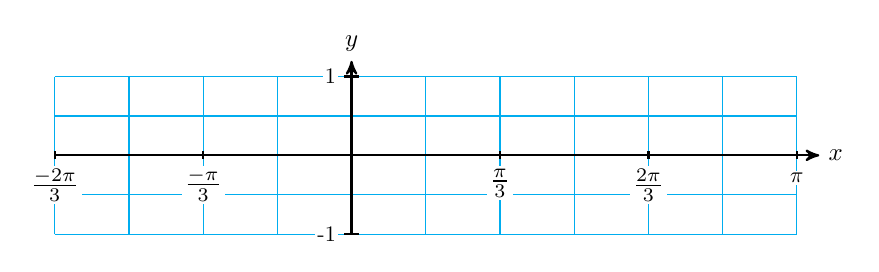
\begin{tikzpicture} [xscale=1.8]
\draw[cyan] (-2*pi/3,-1) grid[xstep=pi/6, ystep=1/2] (pi,1);
\draw[black,thick,->,>=stealth'] (-2*pi/3,0)--(3.3,0) node[right, scale=.9] {$x$};
\draw[black,thick,->,>=stealth'] (0,-1)--(0,1.2) node[above, scale=.9] {$y$};
\draw[black,thick] (-2*pi/3,.05)--++(0,-.1) node[below, yshift=-2, fill=white, inner sep=1] {$\frac{-2\pi}{3}$};
\draw[black,thick] (-pi/3,.05)--++(0,-.1) node[below, yshift=-2, fill=white, inner sep=1] {$\frac{-\pi}{3}$};
\draw[black,thick] (pi/3,.05)--++(0,-.1) node[below, yshift=-2, fill=white, inner sep=1] {$\frac{\pi}{3}$};
\draw[black,thick] (2*pi/3,.05)--++(0,-.1) node[below, yshift=-2, fill=white, inner sep=1] {$\frac{2\pi}{3}$};
\draw[black,thick] (pi,.05)--++(0,-.1) node[below, yshift=-4, fill=white, inner sep=1, scale=.8] {$\pi$};
\foreach \y in {-1,1} \draw[black,thick] (.05,\y)--++(-.1,0) node[left, xshift=-2, fill=white, inner sep=1, scale=.8] {\y};
\end{tikzpicture}
\newline



hp7-sum-13ans $y=\sin\left(\frac{x}{2}+\frac{\pi}{6} \right)$

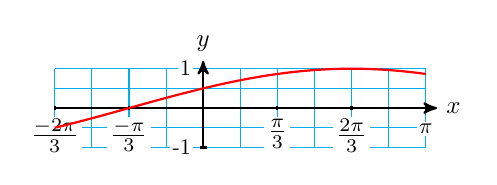
\begin{tikzpicture} [xscale=.9, yscale=.5]
\draw[cyan] (-2*pi/3,-1) grid[xstep=pi/6, ystep=1/2] (pi,1);
\draw[black,thick,->,>=stealth'] (-2*pi/3,0)--(3.3,0) node[right, scale=.9] {$x$};
\draw[black,thick,->,>=stealth'] (0,-1)--(0,1.2) node[above, scale=.9] {$y$};
\draw[black,thick] (-2*pi/3,.05)--++(0,-.1) node[below, yshift=-2, fill=white, inner sep=1] {$\frac{-2\pi}{3}$};
\draw[black,thick] (-pi/3,.05)--++(0,-.1) node[below, yshift=-2, fill=white, inner sep=1] {$\frac{-\pi}{3}$};
\draw[black,thick] (pi/3,.05)--++(0,-.1) node[below, yshift=-2, fill=white, inner sep=1] {$\frac{\pi}{3}$};
\draw[black,thick] (2*pi/3,.05)--++(0,-.1) node[below, yshift=-2, fill=white, inner sep=1] {$\frac{2\pi}{3}$};
\draw[black,thick] (pi,.05)--++(0,-.1) node[below, yshift=-4, fill=white, inner sep=1, scale=.8] {$\pi$};
\foreach \y in {-1,1} \draw[black,thick] (.05,\y)--++(-.1,0) node[left, xshift=-2, fill=white, inner sep=1, scale=.8] {\y};
\draw[samples=65,domain=-2*pi/3:pi, variable=\t, smooth, red, thick] plot (\t,{sin(deg(\t/2 + pi/6) )});
\end{tikzpicture}
\newline



hp7-sum-14 grid 

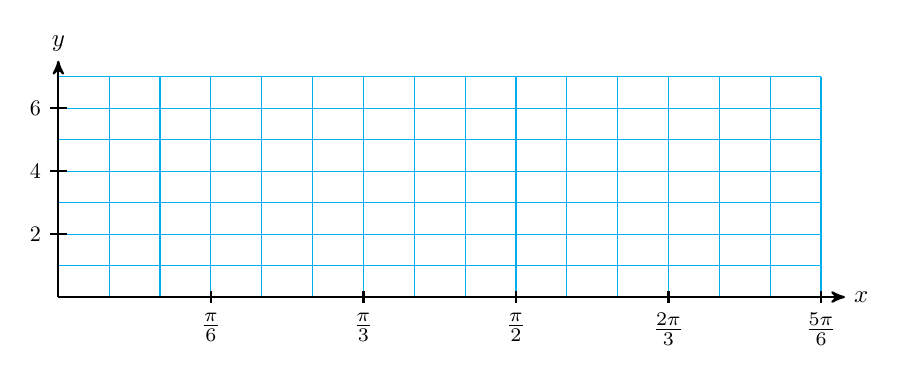
\begin{tikzpicture} [xscale=3.7, yscale=.4]
\draw[cyan] (0,0) grid[xstep=pi/18] (5*pi/6,7);
\draw[black,thick,->,>=stealth'] (0,0)--(2.7,0) node[right, scale=.9] {$x$};
\draw[black,thick,->,>=stealth'] (0,0)--(0,7.5) node[above, scale=.9] {$y$};
\draw[black,thick] (pi/6,.2)--++(0,-.4) node[below, yshift=-2, fill=white, inner sep=1] {$\frac{\pi}{6}$};
\draw[black,thick] (pi/3,.2)--++(0,-.4) node[below, yshift=-2, fill=white, inner sep=1] {$\frac{\pi}{3}$};
\draw[black,thick] (pi/2,.2)--++(0,-.4) node[below, yshift=-2, fill=white, inner sep=1] {$\frac{\pi}{2}$};
\draw[black,thick] (2*pi/3,.2)--++(0,-.4) node[below, yshift=-2, fill=white, inner sep=1] {$\frac{2\pi}{3}$};
\draw[black,thick] (5*pi/6,.2)--++(0,-.4) node[below, yshift=-2, fill=white, inner sep=1] {$\frac{5\pi}{6}$};
\foreach \y in {2,4,6} \draw[black,thick] (.03,\y)--++(-.06,0) node[left, xshift=-2, fill=white, inner sep=1, scale=.8] {\y};
\end{tikzpicture}
\newline



hp7-sum-15 grid 

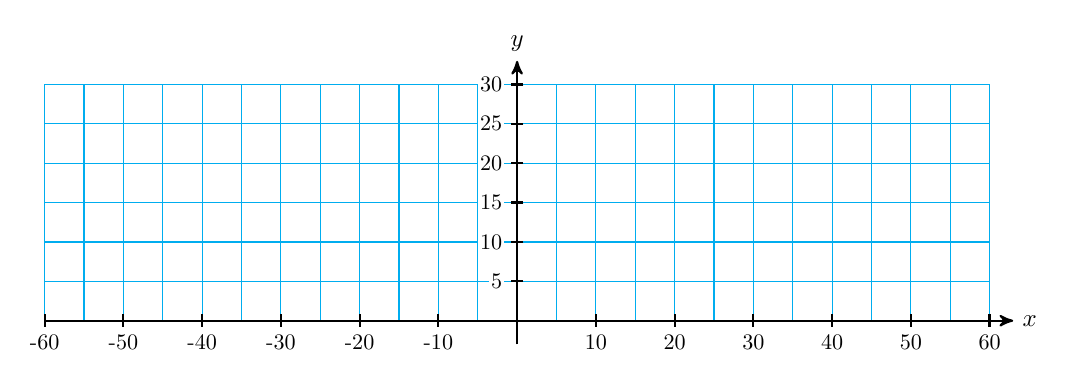
\begin{tikzpicture} [scale=0.1]
\draw[cyan] (-60,0) grid[step=5] (60,30);
\draw[black,thick,->,>=stealth'] (-60,0)--(63,0) node[right, scale=.9] {$x$};
\draw[black,thick,->,>=stealth'] (0,-3)--(0,33) node[above, scale=.9] {$y$};
\foreach \x in {-60,-50,...,-10,10,20,...,60} \draw[black,thick] (\x,.8)--++(0,-1.6) node[below, yshift=-2, fill=white, inner sep=1, scale=.8] {\x};
\foreach \y in {5,10,...,30} \draw[black,thick] (.8,\y)--++(-1.6,0) node[left, xshift=-2, fill=white, inner sep=1, scale=.8] {\y};
\end{tikzpicture}
\newline



hp7-sum-15and $20-5\cos\left(\frac{\pi}{30}x\right)$ 

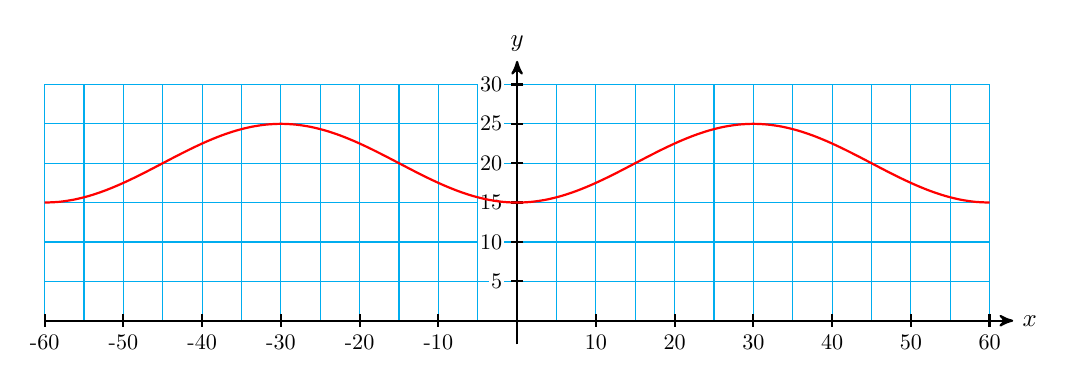
\begin{tikzpicture} [scale=0.1]
\draw[cyan] (-60,0) grid[step=5] (60,30);
\draw[black,thick,->,>=stealth'] (-60,0)--(63,0) node[right, scale=.9] {$x$};
\draw[black,thick,->,>=stealth'] (0,-3)--(0,33) node[above, scale=.9] {$y$};
\foreach \x in {-60,-50,...,-10,10,20,...,60} \draw[black,thick] (\x,.8)--++(0,-1.6) node[below, yshift=-2, fill=white, inner sep=1, scale=.8] {\x};
\foreach \y in {5,10,...,30} \draw[black,thick] (.8,\y)--++(-1.6,0) node[left, xshift=-2, fill=white, inner sep=1, scale=.8] {\y};
\draw[samples=65,domain=-60:60, variable=\t, smooth, red, thick] plot (\t,{20-5*cos(deg(pi*\t/30) )});
\end{tikzpicture}
\newline



hp7-sum-16 grid 

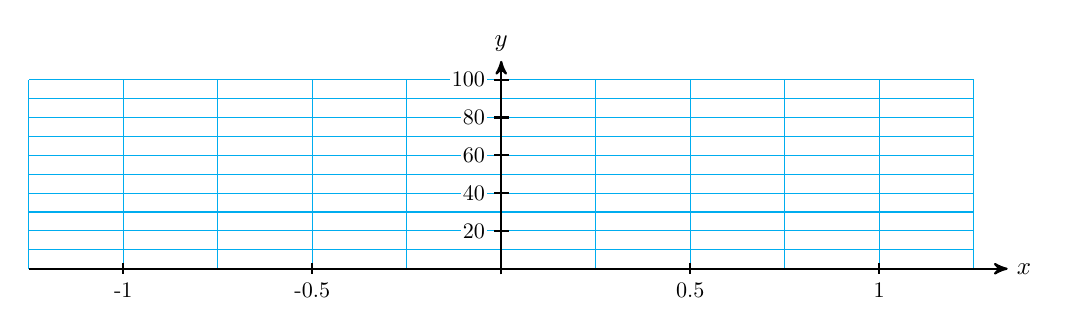
\begin{tikzpicture} [xscale=4.8, yscale=0.024]
\draw[cyan] (-5/4,0) grid[xstep=1/4, ystep=10] (5/4,100);
\draw[black,thick,->,>=stealth'] (-1.25,0)--(1.34,0) node[right, scale=.9] {$x$};
\draw[black,thick,->,>=stealth'] (0,-3)--(0,110) node[above, scale=.9] {$y$};
\foreach \x in {-1,-0.5, 0.5,1} \draw[black,thick] (\x,3)--++(0,-6) node[below, yshift=-2, fill=white, inner sep=1, scale=.8] {\x};
\foreach \y in {20,40,...,100} \draw[black,thick] (.02,\y)--++(-.04,0) node[left, xshift=-2, fill=white, inner sep=1, scale=.8] {\y};
\end{tikzpicture}
\newline


hp7-sum-17 $\frac{1}{4}\sin(\frac{x}{6})+\frac{1}{2}$

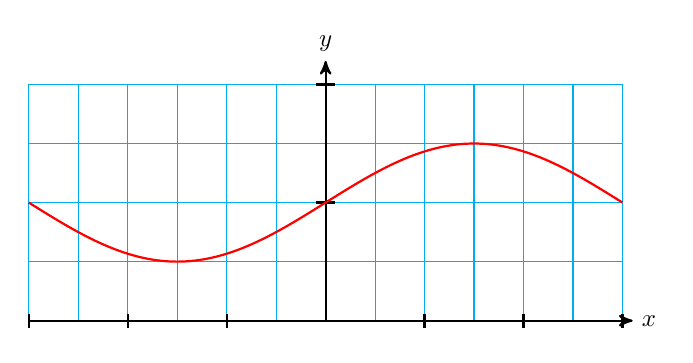
\begin{tikzpicture} [xscale=.2, yscale=3]
\draw[cyan] (-6*pi,0) grid[xstep=pi, ystep=1/4] (6*pi,1);
\draw[black,thick,->,>=stealth'] (-6*pi,0)--(19.5,0) node[right, scale=.9] {$x$};
\draw[black,thick,->,>=stealth'] (0,0)--(0,1.1) node[above, scale=.9] {$y$};
\foreach \x [evaluate=\x as \xi using (pi*\x)] in {-6,-4,-2,2,4,6}  \draw[black,thick] (\xi,.03)--++(0,-.06) ;
\foreach \y in {0.5,1} \draw[black,thick] (.6,\y)--++(-1.2,0);
\draw[samples=65,domain=-6*pi:6*pi,variable=\x, smooth, red, thick] plot (\x,{ 1/4*sin(deg(\x/6) ) +1/2 });
\end{tikzpicture}
\newline


hp7-sum-17ans $\frac{1}{4}\sin(\frac{x}{6})+\frac{1}{2}$

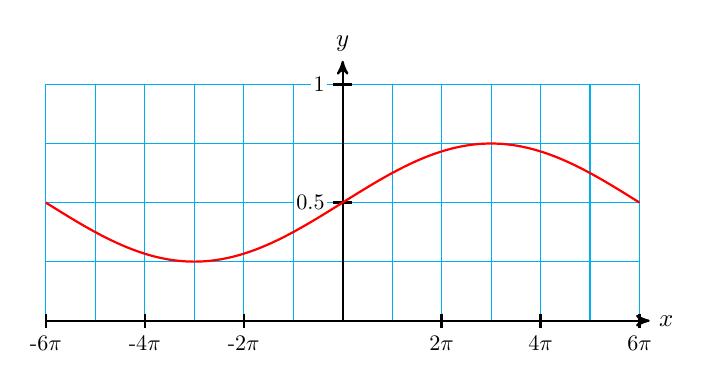
\begin{tikzpicture} [xscale=.2, yscale=3]
\draw[cyan] (-6*pi,0) grid[xstep=pi, ystep=1/4] (6*pi,1);
\draw[black,thick,->,>=stealth'] (-6*pi,0)--(19.5,0) node[right, scale=.9] {$x$};
\draw[black,thick,->,>=stealth'] (0,0)--(0,1.1) node[above, scale=.9] {$y$};
\foreach \x [evaluate=\x as \xi using (pi*\x)] in {-6,-4,-2,2,4,6}  \draw[black,thick] (\xi,.03)--++(0,-.06) node[below, yshift=-2, fill=white, inner sep=1, scale=.8] {\x$\pi$};
\foreach \y in {0.5,1} \draw[black,thick] (.6,\y)--++(-1.2,0) node[left, xshift=-2, fill=white, inner sep=1, scale=.8] {\y};
\draw[samples=65,domain=-6*pi:6*pi,variable=\x, smooth, red, thick] plot (\x,{ 1/4*sin(deg(\x/6) ) +1/2 });
\end{tikzpicture}
\newline


hp7-sum-18 $\frac{3}{2}\cos(\frac{x}{2})-2$

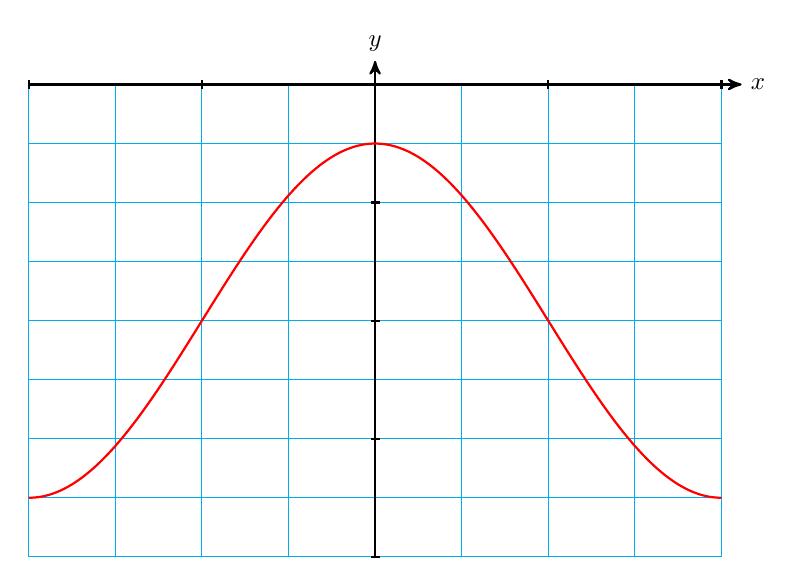
\begin{tikzpicture} [xscale=.7, yscale=3/2]
\draw[cyan] (-2*pi,-4) grid[xstep=pi/2, ystep=1/2] (2*pi,0);
\draw[black,thick,->,>=stealth'] (-2*pi,0)--(6.65,0) node[right, scale=.9] {$x$};
\draw[black,thick,->,>=stealth'] (0,-4)--(0,0.2) node[above, scale=.9] {$y$};
\foreach \x [evaluate=\x as \xi using (pi/2*\x)] in {-4,-2,2,4}  \draw[black,thick] (\xi,.04)--++(0,-.08) ;
\foreach \y in {-4,-3,-2,-1} \draw[black,thick] (.08,\y)--++(-.16,0);
\draw[samples=65,domain=-2*pi:2*pi,variable=\x, smooth, red, thick] plot (\x,{ 3/2*cos(deg(\x/2) ) -2 });
\end{tikzpicture}
\newline


hp7-sum-19ans $y=-5\cos (2x-0.5)+3$

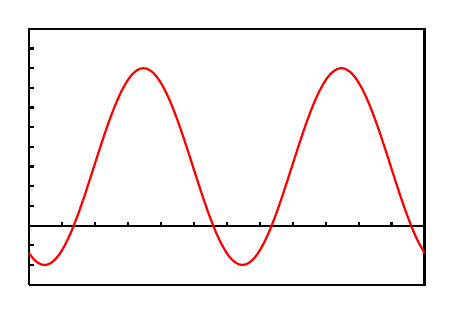
\begin{tikzpicture} [xscale=.8, yscale=.25]
\draw[black,thick] (0,-3) --++(2*pi,0) --++(0,13)--++(-2*pi,0) --++(0,-13);
\draw[black,thick] (0,0)--(2*pi,0);
\draw[black,thick] (0,-3)--(0,10);
\foreach \x [evaluate=\x as \xi using (\x*pi /6)] in {1,2,...,12}  \draw[black,thick] (\xi,.2)--++(0,-.2) ;
\foreach \y in {-3,-2,...,10} \draw[black,thick] (.08,\y)--++(-.08,0);
\draw[samples=65,domain=0:2*pi,variable=\x, smooth, red, thick] plot (\x,{ -5*cos(deg(2*\x -0.5) ) +3 });
\end{tikzpicture}
\newline





\end{document}
